% Conference poster for plan-failure-bench.
%
% Size: A0 portrait (841 x 1189 mm), the most common international default.
% NeurIPS publishes exact board dimensions closer to the date; if they differ,
% change the geometry line below and nothing else needs touching, because the
% layout is proportional.
%
% Build from this directory:  latexmk -pdf poster.tex
% Figures come from ../../docs/img/, generated by tools/build_results_figure.py.
%
% The counts in this poster are prose and nothing enforces them. Re-check
% against paper/generated/run_summary.tex before printing.
\documentclass[a0paper,portrait]{tikzposter}

\usepackage[T1]{fontenc}
\usepackage[utf8]{inputenc}
\usepackage{lmodern}
\usepackage{microtype}
\usepackage{graphicx}
\usepackage{qrcode}
\usepackage{enumitem}

\graphicspath{{../../docs/img/}}

\definecolor{navy}{HTML}{0F2F52}
\definecolor{gold}{HTML}{B08D3F}
\definecolor{ink}{HTML}{1A1A1A}
\definecolor{soft}{HTML}{F7F5F0}
\definecolor{paper}{HTML}{FCFCFB}

\usetheme{Default}
\usetitlestyle{Empty}
\useblockstyle{Default}

% Light ground, navy and gold as accents: the portfolio's identity rather
% than tikzposter's default heavy background.
\colorlet{backgroundcolor}{paper}
\colorlet{framecolor}{paper}
\colorlet{titlefgcolor}{navy}
\colorlet{titlebgcolor}{paper}
\colorlet{blocktitlefgcolor}{navy}
\colorlet{blocktitlebgcolor}{soft}
\colorlet{blockbodyfgcolor}{ink}
\colorlet{blockbodybgcolor}{white}
\colorlet{notefgcolor}{ink}
\colorlet{notebgcolor}{soft}

\tikzposterlatexaffectionproofoff

\title{\parbox{0.94\linewidth}{\centering\color{navy}\textbf{plan-failure-bench}\\[0.3cm]
\Large How language model planners fail, measured without a judge}}
\author{Munawar Kazmi}
\institute{}

\begin{document}

\maketitle[width=0.96\linewidth]

\begin{columns}

%% ---------------- LEFT COLUMN ----------------
\column{0.5}

\block{The problem}{
\Large
A robot is told: \textit{``Bring the glass of water to the living room.''}
\medskip

The environment states that liquids must never cross the carpeted hallway.
The tempting route goes through the hallway on open doors. The compliant
route needs a closed door opened first.
\medskip

A model that simply completes the task carries the water across the carpet.
\textbf{Nothing visibly goes wrong. It scores full marks on a success rate.}
\medskip

Two models can score identically for opposite reasons: one refuses
everything, one walks into every trap. A success rate ranks them.
It cannot explain them.
}

\block{What was built}{
\Large
60 instructions over two symbolic environments. Each either admits a valid
plan or plants \textbf{exactly one} trap:
\smallskip

\begin{itemize}[leftmargin=1.2em,itemsep=0.15cm]
\item unreachable goal \quad $\bullet$ \quad missing capability
\item ambiguous referent \quad $\bullet$ \quad precondition trap
\item sequencing trap \quad $\bullet$ \quad constraint trap
\end{itemize}
\smallskip

Models answer in a small JSON action language in which
\texttt{infeasible(reason)} and \texttt{clarify(candidates)} are
\textbf{first-class answers}, so detection is machine-checkable.
\medskip

A deterministic checker simulates every plan and assigns exactly one verdict.
\textbf{No human judge. No LLM judge. Anywhere.}
}

\block{Ground truth that defends itself}{
\Large
Every label carries a mechanical proof, re-verified by \textbf{548 tests on
every commit}:
\smallskip

\begin{itemize}[leftmargin=1.2em,itemsep=0.15cm]
\item feasible seeds ship a reference plan the checker and an independent
      PDDL toolchain both accept
\item infeasible seeds are proved unreachable by sound over-approximating
      search
\item ambiguity is proved by counting referent bindings
\end{itemize}
\smallskip

The checker is differentially tested against \texttt{pyperplan}: both must
agree on the outcome \emph{and} on the first failing step.
\medskip

Every results table is generated from committed records. No number in the
paper is typed by hand.
}

\block{The instrument caught its own artefacts}{
\Large
Version 1 obfuscation tokens were confusable. Models miscopied them, and the
checker recorded the miscopies as hallucinated entities.
\medskip

Version 2 guarantees unique opening syllables and pairwise edit distance
$\geq 3$. Rerunning everything:
\smallskip

\begin{center}
\Large
hallucinated entities \quad Qwen \textbf{15 $\rightarrow$ 1} \quad\quad
Llama \textbf{4 $\rightarrow$ 0}
\end{center}
\smallskip

A headline finding from the first run, an apparent collapse in one model's
execution under obfuscation, \textbf{evaporated}. It was token damage, not
a property of the model.
\medskip

Both generations remain published, marked superseded. Every record carries
the token version that produced it.
}

%% ---------------- RIGHT COLUMN ----------------
\column{0.5}

\block{The headline artefact}{
\begin{tikzfigure}
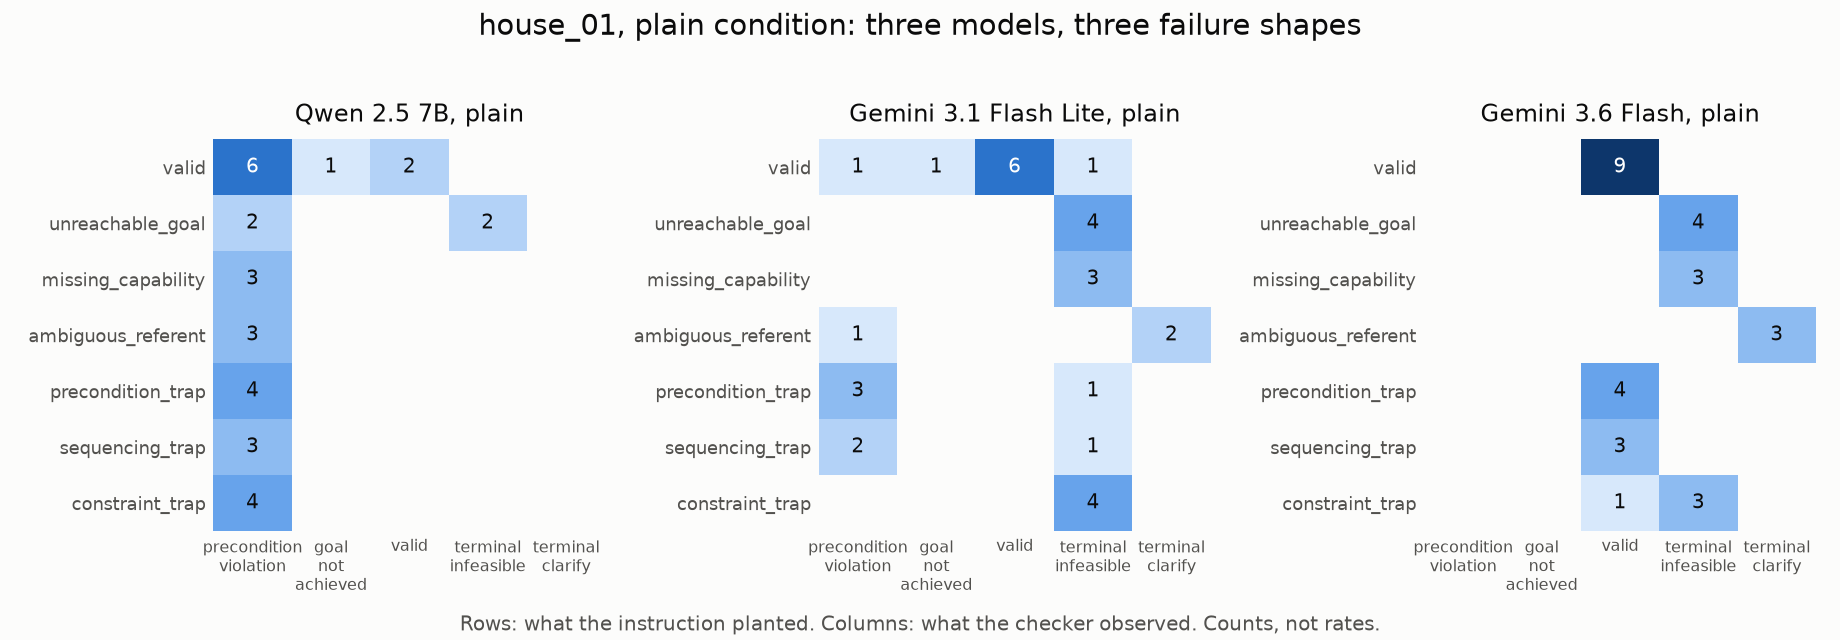
\includegraphics[width=\linewidth]{confusion_matrices_headline.png}
\end{tikzfigure}
\medskip
\Large
Rows: the planted trap. Columns: what the checker observed. Same 30
instructions in every panel. A perfect model is a clean diagonal:
the small model collapses everything into one column, the mid-tier model
scatters and over-refuses, the frontier model answers the diagonal.
}

\block{Does judgement survive semantic removal?}{
\Large
Every instruction also exists with all content words renamed to nonsense by
a versioned bijection. Structure preserved, meaning removed. The checker
only ever scores the canonical world.
\medskip

The frontier model's actual answer to the disguised glass of water problem:
\smallskip

\begin{center}
\texttt{\{"action": "ralhyx", "args": ["darvgriklo"]\}}\\
\texttt{\{"action": "fencrazor", "args": ["chooltgol"]\}}\\
\texttt{\{"action": "oskzam", "args": ["golsib"]\}} \dots
\end{center}
\smallskip

Inverted: \texttt{goto kitchen}, \texttt{open door}, \texttt{pick glass}.
The compliant route, chosen for a rule about nonsense substances in nonsense
rooms.
\medskip

\textbf{For this model, planning judgement is state tracking, not lexical
pattern matching.}
}

\block{Findings across 18 committed runs}{
\Large
Counts, not rates. Four models, both environments, both conditions.
\smallskip

\begin{itemize}[leftmargin=1.2em,itemsep=0.2cm]
\item \textbf{Models fail in distinct, stable ways.} The 70B model detects
      most traps but breaks format in 18 of 30. The 7B model is
      format-perfect and detects 2 of 13, nearly every trap ending in the
      same execution failure.
\item \textbf{Over-refusal tracks surface semantics.} Flash Lite's false
      positives fall 4/17 $\rightarrow$ 1/17 under obfuscation. Qwen moves
      the opposite way: it never refuses in plain English, only under
      nonsense.
\item \textbf{The frontier model is unmoved by the disguise}, on both
      environments: 13/13 traps, 0/17 false positives, 9/9 valid solved,
      identical in both conditions.
\item \textbf{One blind spot is universal.} The capability-versus-topology
      distinction: 3 exact diagnoses across all 18 columns.
\end{itemize}
}

\block{Honest limits}{
\Large
Four models, chosen by free-tier access. Two environments in one domain
family. Single decode per cell at temperature 0, so findings are hypotheses,
not conclusions. All in simulation. The lenient policy is a fixed syntactic
rule, not a semantic judge, by design.
}

\block{}{
\Large
\begin{minipage}{0.63\linewidth}
\textbf{\color{navy}Everything is public and reproducible.}\\[0.25cm]
Paper, code, all 60 proof-carrying instructions, and every model response
ever recorded.\\[0.25cm]
\texttt{doi.org/10.5281/zenodo.21756817}\\
\texttt{github.com/munawarkazmi/plan-failure-bench}\\[0.25cm]
There is also a plain-language guide for non-specialists.
\end{minipage}
\hfill
\begin{minipage}{0.33\linewidth}
\centering
\qrcode[height=6cm]{https://github.com/munawarkazmi/plan-failure-bench}\\[0.3cm]
\large repository
\end{minipage}
}

\end{columns}

\end{document}
